% !TeX root = ../main.tex
% Add the above to each chapter to make compiling the PDF easier in some editors.

\chapter{Evaluation}\label{chapter:Evaluation}

The goal of this chapter is to validate the framework architecture design for context-aware pervasive computing in challenged environments which was described in Chapter \ref{chapter:Approach}. It also evaluates the middleware implementation which was explained in Chapter \ref{chapter:implementation}. Note that, the delays and performances are to be taken with a grain of salt, as the system is designed as a proof-of-concept and not to run in production systems. \\

\noindent To satisfy all the requirements and specification for the software framework, we divided the evaluation into several sections. Each section validates certain specification via implementing a use case scenario. We describe which requirements where targeted at the beginning of each section.
The devices used for  the use cases have different hardware capabilities. They might also have  sensors and actuators according to each use case. All the devices must be running our stack framework as explained in \ref{subsec:starting-framework} except for android phones which has \textit{Liberouter}, an implementation for SCAMPI on android phones. The devices we used in this evaluation are:
\begin{table}[!ht]
	\centering
	\begin{tabular}{*{4}{c}}\toprule
		Name & Count & Stack & Performance \\ \hline
		 &  &  &  \\
		Intel NUC &1& 	Our framework &   \specialcell[c]{CPU:Intel Core i5-6260U Processor\\ (4M Cache, up to 2.90 GHz)\\RAM: 16GB }\\ 
		&  &  &  \\
		Raspberry Pi 3 model B & 2 & Our framework &  \specialcell[c]{ CPU: 1.2GHz\\RAM: 1GB}  \\ 
		&  &  &  \\
		HTC One M9 & 1 & Liberouter &   \specialcell[c]{CPU: Octa-core \\4 x 2.0GHz + 4 x 1.5GHz\\ RAM: 3GB} \\ \hline

\end{tabular}
\caption{Devices used for the implementation evaluation.}
\label{table:devoces}
\end{table}

\section{Basic IoT Usage}

First, we wanted to evaluate that the software framework works with the basic IoT use cases using high rate data sensors and storing them in time-series database. The flow explained in \ref{susbec:temp}  reads temperature on a regular time basis and stores it into a database, it also has an endpoint that can query for data between specific time intervals and if no time interval is specified, it will return temperature readings in the last two minutes. The flow also alerts for high temperatures by igniting a red led lamp. \\

\noindent The use case is an example of pervasive computing that checks if the temperature is above certain degree and then act by lighting the red led. It also serves as an abstraction for other use cases with real life purposes. For example, we might have a goal to start or close an air conditioning system in a building according to the temperature., Thus, the flow can be adjusted to include an API for the air conditioning system instead of lighting a red led. The use case can also be extended to include a monitoring system, that can show temperatures collected from different devices. Further, it can include location information along with the temperature data thus knowing what are the temperatures in different locations by syncing database instance on each device to the cloud.\\

\noindent In this experiment we used a two Raspberry Pis running our proposed stack that are connected along with a switch and router. The publishing PC is connected to the network through the router via Wi-Fi as shown in \ref{fig:tb-temp} . First, a PC sends the flow for temperature reading, data storage and creating an endpoint to query the data. Then, once the flow is received and deployed, the temperature sensors starts gathering temperatures and stores it into a local database. 

 \begin{figure}[H]
	\centering
	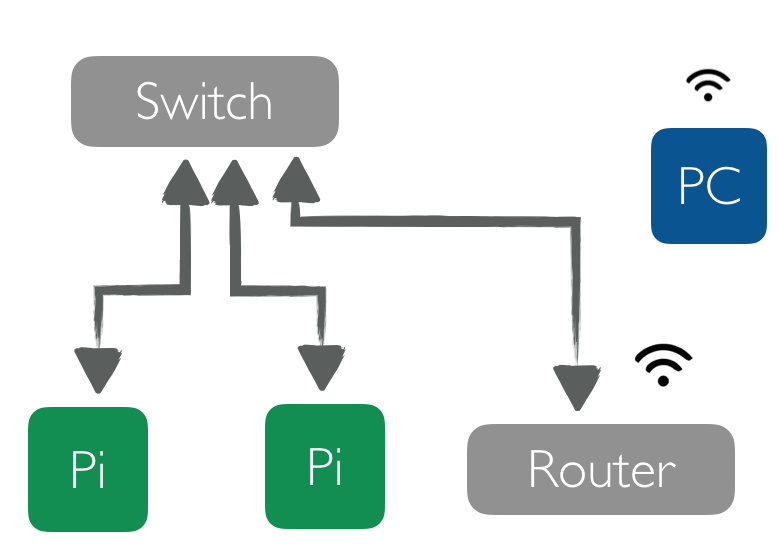
\includegraphics[scale=0.6]{images/tb-temp.png}
	\caption{Testbed setup for temperature sensing flow.}
	\label{fig:tb-temp}
\end{figure} 

\noindent The experiment was run 8 times and each time  we measured the delay between publishing the flow from the PC $ t_{PC}$ till it is received and deployed by  node-RED instances on the Raspberry Pis $t_{PI}$, we also measured the delay between flow deployment and the first database temperature insert query on the device's instance $t_{db}$. 
\begin{table}[H]
	\centering
	\begin{tabular}{*{5}{c}}\toprule
		&  $ t_{Pi1} - t_{PC}$   & $t_{db} - t_{Pi1}$  & $ t_{Pi2} - t_{PC}$ &  $t_{db2} - t_{Pi2}$ \\ \midrule
meant &2.870&	1.723&	2.437&	1.717\\
standard deviation& 0.769	&0.0376&	1.003&	0.013\\
	\end{tabular}
	\caption{Results, mean and standard deviation of temperature flow delays.}
	\label{table:temp}
\end{table}

\noindent Given these delays, the average time a temperature flow takes to reach the Raspberry Pi and gets deployed is 2.653 seconds , the average time till the first temperature insert in the database    is 1.720 seconds. Which means that in our proof-of-concept implementation, it takes on average 4.373 seconds from the moment a flow  which can sense the environment and stores data into a database till the first metric insertion is done.


\section{Recognizing Water Bottles } \label{sec:rwb}


Moving on to more complex scenarios, This use case  is as follows, movements are detected around low computation devices portrayed as the Raspberry Pis. Once they detect movements around them, they take an image and send it to the topic \textit{NUC}. A high performance machine "an Intel NUC" should be waiting for input on the same topic. As soon as the NUC  receives an image, it runs an image recognition algorithm and responds back to the Raspberry Pi which sent the original message  only if the recognizer recognizes a water bottle. When a Raspberry Pi receives the recognition result on its endpoint, this means that the image was a watter bottle with a certain confidence, therefore, the Pi signals a red led to light up and stores the result in a database. \\ 

\noindent The flows implementation used to create this use case can be found in \ref{subsec:tensor} and \ref{subsec:detect-move}.  As part of this experiment when a flow requiring high amount of performance such as the image recognition flow is received by low performing devices they will not get deployed and  will log that requirements were not satisfied. The same case applies when a flow requiring low amount of computing power is received by a high performing device, of course, this could be optimized because clearly high performance devices can execute flows which are not needy. The computational requirements needed by each flow are decided before sending the flow over to other devices using the HTML page implemented in the publishing flow explained in \ref{subsec:send-comp}.\\ 

This scenario helps us validate several requirements for the software framework evaluation: 
\begin{enumerate}
	\item Sending flows to all nodes connected to a network  running our framework stack.
	\item Controlling which devices can deploy the flows by sending meta-data for the resources and computation power along with flow. Therefore, being able to only send to some sets of nodes.
	\item Checking requirements of flows and rejecting the deployment if they were not satisfied at the receiving devices.
	\item Sending data or flows to a  specific node using its global identifier.
	\item Carrying flow dependencies in order to guarantee a successful run at the receiving node.
\end{enumerate}

\noindent As stated every device must have the framework stack running before we start our use case. So after making sure its running we start publishing the flows. In this use case, the testbed setup is shown in figure \ref{fig:tb-tensor}, it consists of two Raspberry Pis, an Intel NUC and a router connected via switch. The PC which will publish the computations is connected through the router via WI-FI. 
 \begin{figure}[H]
	\centering
	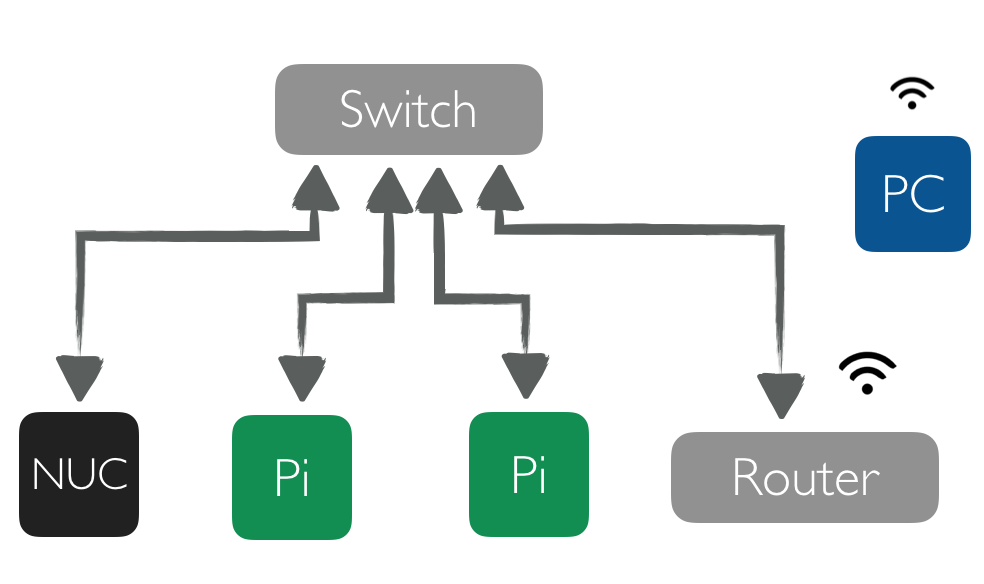
\includegraphics[scale=0.6]{images/tb-tensor.png}
	\caption{Testbed setup for recognizing water bottles.}
	\label{fig:tb-tensor}
\end{figure} 



\noindent We started by publishing the flow \ref{subsec:tensor} for  image recognition with all its dependencies in total 83MB, then we published the motion detection flow \ref{subsec:detect-move} with the sensor scripts. We measured the delay between publishing flows from the PC till it was received and deployed by node-RED on each instance. The use case was run 8 times, we also measured the delay when a motion was detected by Raspberry Pi and an image was sent to the NUC and the recognizer reply, this was also run 8 times for each Pi, a total of 16 runs. The sequence diagram shown in \ref{fig:sd-tensor},  illustrates the procedure in addition to the time initials for each part of the process.  \\



\begin{figure}[H]
	\centering
	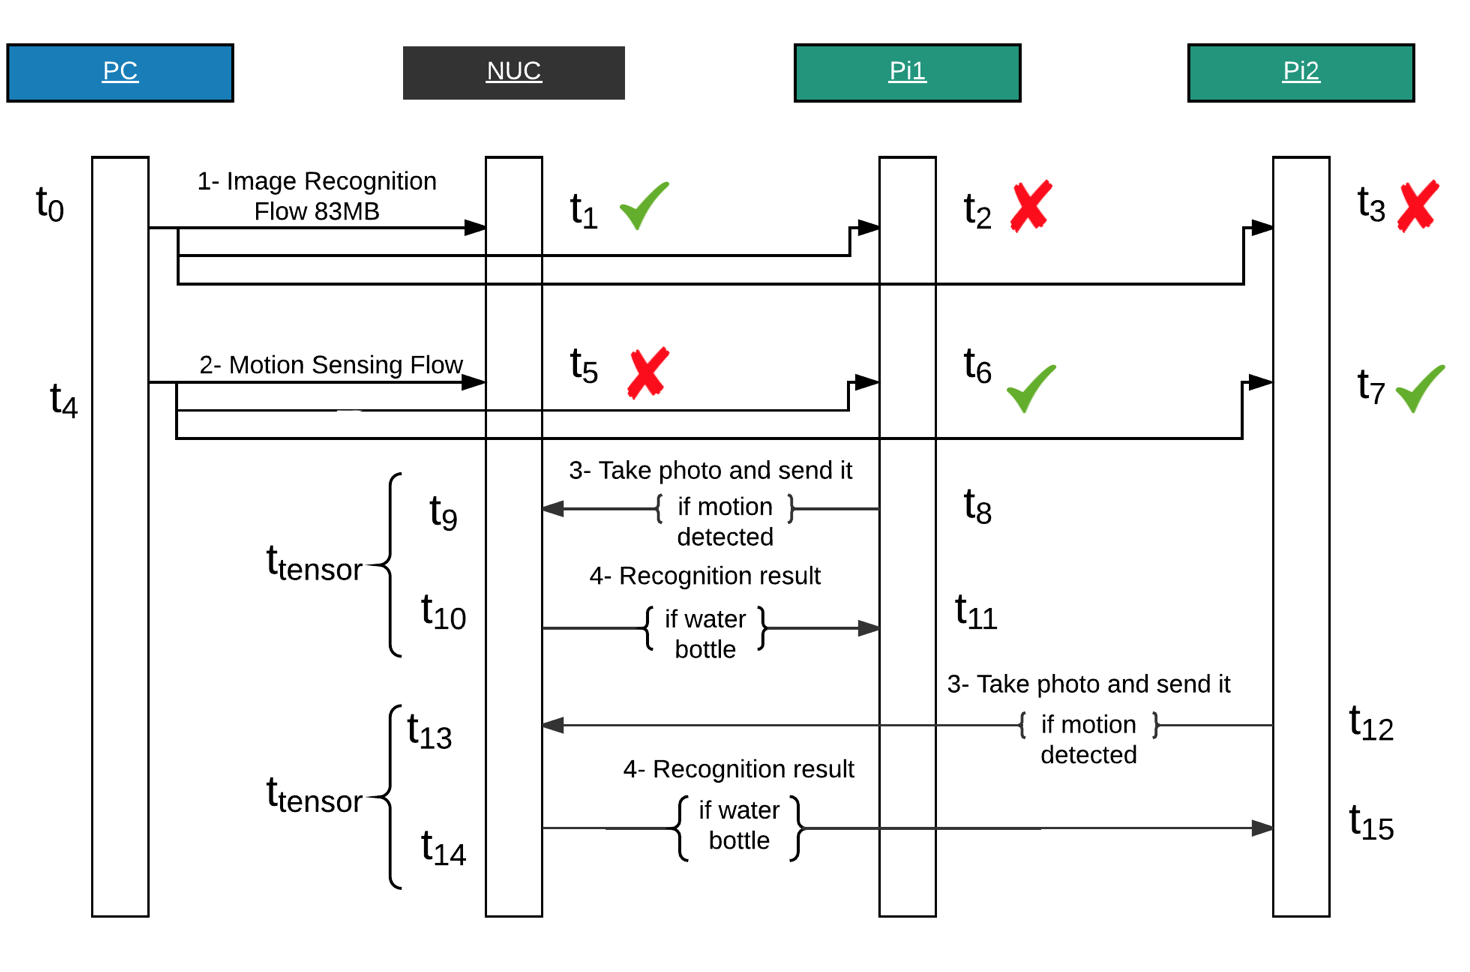
\includegraphics[scale=0.45]{images/sequence-diagram.png}
	\caption{Sequence diagram for recognizing water bottles.}
	\label{fig:sd-tensor}
\end{figure} 
 


\noindent At time $t_0$ the image recognition flow was published, at times $t_1, t_2$ and   $t_3$ it was received by the NUC, Pi1 and Pi2 respectively. Then at time $t_4$ the motion sensing flow was published and at times $t_5,t_6$ and $ßt_7$ it was received by the other devices as well. A times $t_8$ and $t_{12}$  the Pis detected motion, took an image and then sent a message to the NUC. At times $t9$ and $t{13}$,  NUC received messages from the Pis and started processing, detected a watter bottle and then sent the  results back to the senders at $t_{10}$ and $t_{14}$. The Pis received recognition responses with the confidence percentage at $t_{11}$ and $t_{12}$.  The tables \ref{table:tensor}, \ref{table:motion} and \ref{table:data} show the mean and standard deviation of the delays.  
\begin{table}[H]
\centering
\begin{tabular}{*{4}{c}}\toprule
&$t_1 - t_0$  & $t_2 - t_0$  & $t_3-t_0$ \\ \midrule
1&	23.245&	28.226&	20.826\\
2&	20.699&	49.666&	19.051\\
3&	22.330&	21.756&	29.425\\
4&	21.387&	22.265&	32.680\\
5&	22.549&	27.662&	22.627\\
6&	24.095&	27.222&	15.922\\
7&	19.597&	25.561&	43.311\\
8&	22.586&	26.898&	28.627\\
mean&	23.245 s&28.226 s&20.826 s\\ 
standard deviation &1.440 s&8.830 s&8.851 s\\
\end{tabular}
\caption{Results, mean and standard deviation of the image recognition flow delays.}
\label{table:tensor}
\end{table}


\begin{table}[H]
\centering
\begin{tabular}{*{4}{c}}\toprule
&$t_5 - t_4$  & $t_6 - t_4$  & $t_7-t_4$ \\ \midrule
1&	0.104&	2.386&	2.233\\
2&	0.106&	2.323&	2.348\\
3&	0.090&	2.321&	1.380\\
4&	0.080&	2.340&	1.275\\
5&	0.076& 2.210&	1.441\\
6&	0.081&	2.299&	2.247\\
7& 0.088&	2.329&	2.211\\
8&	0.074&	2.368&	2.450\\
mean t&0.087 s&2.322 s&1.948 s\\
standard deviation&0.012 s&0.053 s&0.491 s\\
\end{tabular}
\caption{Results, mean and standard deviation of the motion detection flow delays.}
\label{table:motion}
\end{table}

\begin{table}[H]
\centering
\begin{tabular}{*{6}{c}}	\toprule
&$t_9 - t_8$  & $t_{11} - t_{10}$  & $t_{13}-t_{12}$ & $t_{15}-t_{14}$&  $t_{tensor}$ \\ \midrule
1&	0.266&	0.659&	0.276&	0.686&	5.582\\
2&	0.296&	0.674&	0.323&	0.79&	5.640\\
3&	0.186&	0.728&	0.313&	0.676&	5.573\\
4&	0.342&	0.807&	0.222&	0.661&	4.940\\
5&	0.227&	0.752&	0.219&	0.722&	5.603\\
6&	0.262&	0.713&	0.322&	0.742&	5.599\\
7&	0.306&	0.684&	0.212&	0.663&	5.575\\
8&	0.374&	0.582&	0.293&	0.648&	5.581\\
mean&0.282 s&0.700 s&	0.273 s&0.6985 s&5.512 s\\
standard deviation&0.061 s&0.067 s&	0.048 s&0.0488 s&0.217 s\\
	\end{tabular}
	\caption{Results, mean and standard deviation for sending and receiving data delays.}
	\label{table:data}
\end{table}

\noindent It is clear that  delays of the flow carrying image recognition dependencies took long times compared to the motion flow and the data messages between the NUC and Pis. That is mostly because the size of data in which the message is carrying. The data messages included images with size from 50K to 90K  and motion sensing flow had dependencies with size less than 2K. It is also clear that when the receiving side are the Raspberry Pis, delays are usually larger than when the receiving side is the NUC. This is evident in the motion sensing delays \ref{table:motion} and  also in \ref{table:data} despite the message sent from the Raspberry Pis to the NUC are heavier than their replies  in terms of size, but the delays are much less.

\section{Local Composability}
In order to prove that we can compose flows locally using our framework, we created a use case that builds on the  previous experiment. Our goal is to use the same database configuration in both flows, one to write into a database while the other reads. Therefore, being able to compose two flows in order to achieve a bigger use case.\\

 \noindent Continuing on the same test bed setup as \ref{sec:rwb} and same scenario.  After the Raspberry Pis stored the recognized images of water bottles into their respective  databases, we sent a flow that retrieves these images from the database into a web endpoint along with their confidence percentages explained in \ref{subsec:images}. By doing this, we make sure that flows can be locally composed using the same database configuration. We also measured the delay between sending the images flow from the PC until it was deployed by node-RED on other devices. The flow required low computational effort, therefore, ir will not get deployed on the NUC device. The experiment was also run 8 times.

\begin{table}[H]
\centering
\begin{tabular}{ c | c | c| c }	\toprule
&$t_{17} - t_{16}$  & $t_{18} - t_{16}$  & $t_{19}-t_{16}$ \\ \midrule
1&	0.102&	0.761&	0.838\\
2&	0.163&	0.799&	0.799\\
3&	0.125&	0.927&	0.923\\
4&	0.091&	0.752&	0.868\\
5&	0.070&	0.814&	0.778\\
6&	0.095&	0.824&	0.861\\
7& 0.094&	0.736&	0.835\\
8&	0.098&	0.798&	0.769\\	
mean&	0.105&	0.801&	0.834\\
standard deviation&	0.028&	0.060&	0.051\\
\end{tabular}
\caption{Results, mean and standard deviation for retrieving recognized images flow delays.}
\label{table:images}
\end{table}

\noindent Delays in this use case is quite low because this flow does not have any dependencies at all. Comparing the times in which the Raspberry Pi's have received and deployed flows, this one  has quite the least delay. However, the NUC in this flow seemed to have a bit higher delay average than the motion sensing flow with not so much dependencies as well.


\section{Challenged Networks}
In this section, our aim is to evaluate that the framework works in challenged networks with no end-to-end path between  sender and receiver. We used the same setup as \ref{sec:rwb} but with two major changes. The first change is that we disconnected  a Raspberry PI from the network switch, therefore, it is no longer connected to the other devices or the publishing PC, we also set-upped the disconnected node as an access point in which other devices can connect to using Wi-Fi. The second change is that we introduced an android phone that can connect to both the Raspberry Pi's access point and the router's Wi-Fi connected to the switch. Additionally, the device switches it's Wi-Fi between the access point and router Wi-Fi each 80 seconds. The system setup is shown in figure \ref{fig:tb-dtn}.
\begin{figure}[H]
	\centering
	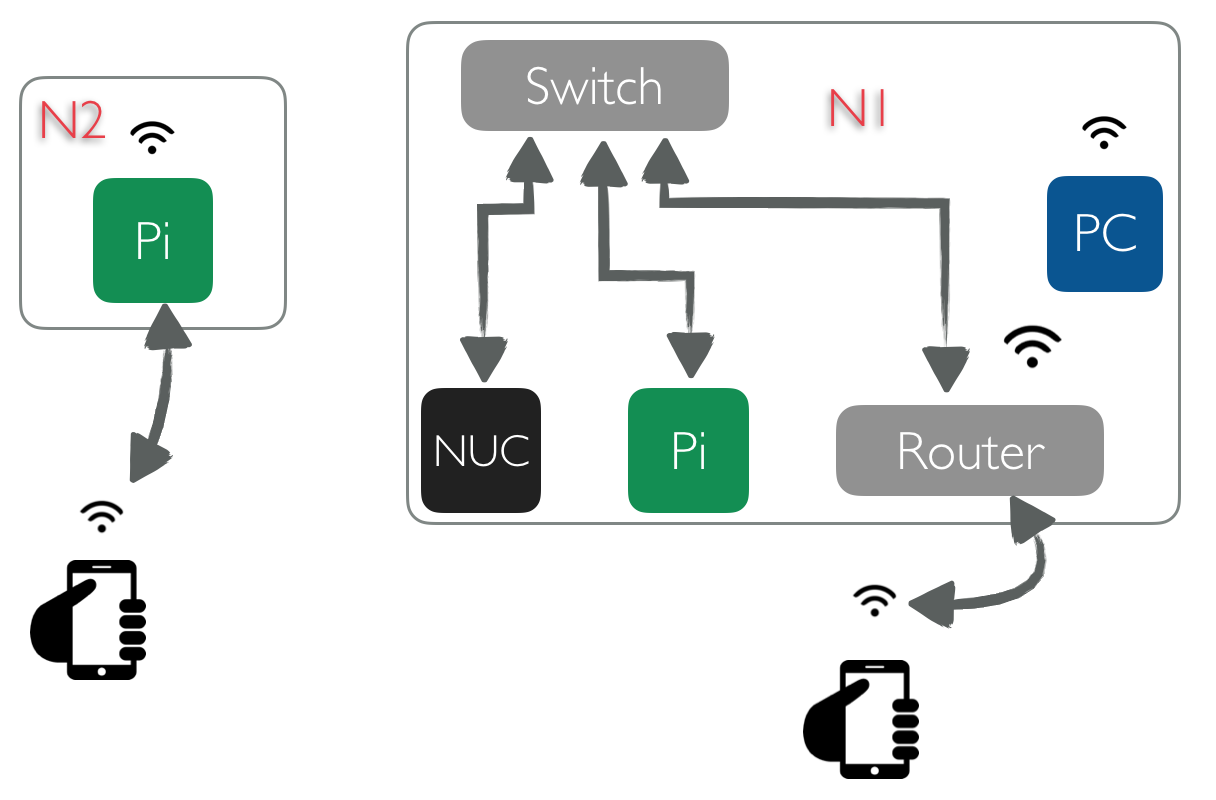
\includegraphics[scale=0.6]{images/tb-dtn.png}
	\caption{Testbed setup for challenged and delay tolerant networks.}
	\label{fig:tb-dtn}
\end{figure} 

\noindent The experiment was run only one time for an extended amount of 50 minutes. First, we used the PC to publish the image recognition flow and the motion sensing flow. Second, we waited some time until we made sure that the flows have reached the disconnected Pi. Afterwards, we passed hands over the infrared sensor of the disconnected Pi and put a water bottle in front of the camera. We repeated this action multiple times.\\

\noindent This use case is evaluated differently, since in this experiment, we do not have a way to map image recognition requests sent from the disconnected Pi to the NUC with their respective responses. Also, there are some recognition requests that was not detected as a water bottle therefore there was no response from the NUC. Thats why we evaluate this use case on 3 different levels. First, the delay between publishing  flows from the PC and receiving them on all devices. Second, the delay between sending the images from the disconnected Pi to the NUC. Third, the delay between sending the result from NUC till it is deployed to the disconnected Pi.  Note that the number of messages sent from the Pi to the NUC and vice versa may not be equal due to the fact that some images were not recognized as water bottles. In addition, we have no means to map a message which was sent as a image recognition request to another one sent as a response which could be future work. \\

\noindent The following table shows the first evaluation phase, $t_{NUC}$, $t_{Pi}$ and $t_{disconnected-pi}$ are the delays between publishing the flows from the PC till it reach each device.
\begin{table}[H]
	\centering
	\begin{tabular}{*{4}{c}}\toprule
		&$t_{NUC}$  & $t_{Pi1}$  & $t_{disconnected-pi}$ \\ \midrule
		image recognition flow& 39.414&	53.719&	312.072s\\
		motion sensing flow&3.163&	5.401&	215.657\\
	\end{tabular}
	\caption{The delays for sending flows to the network devices including the disconnected PI.}
	\label{table:DIS}
\end{table}

\noindent From the above table we can definitely see the delay added to the disconnected Pi. This main reason for that  is, beside not having a direct connection, the switching window of the android device. It can affect the transfer in different ways and has its trade-offs. If the switching time is too big, the delay will most probably increase because after a flow is uploaded to the phone, it will have to wait for some time until the window closes before it switches to the other network. But also, having it too small, flows with  large size of dependencies will not succeed to upload data to the android phone in time. 


Next we show the delays of some messages that were sent from the disconnected Pi to the NUC carrying images with their average and standard deviation.
\begin{table}[H]
	\centering
\begin{tabular}{*{2}{c}}\toprule
		  & $t$  \\ \midrule
1&	284.957\\
2&	216.409\\
3&	180.415\\
4&	228.811\\
5&	228.329\\
6&	220.11\\
7&	214.213\\
8&	111.267\\
9&	104.166\\
10&	101.188\\
11&	179.825\\
12&	178.946\\
13&	166.999\\
mean&	185.818\\
standard deviation&	54.966\\
\end{tabular}
	\caption{Messages delays sent from the disconnected Raspberry Pi to the NUC.}
	\label{table:DIS2}
\end{table}

\noindent Finally, we evaluated the response message returning back from the NUC to the disconnected Raspberry Pi having successfully recognized a water bottle.

\begin{table}[H]
	\centering
	\begin{tabular}{*{2}{c}}\toprule
		& $t$  \\ \midrule
1&	59.531\\
2&	51.51\\
3&	51.826\\
4&	213.212\\
5&	67.856\\
6&	67.673\\
7&	68.188\\
8&	68.103\\
9&	64.292\\
10&	192.479\\
mean& 	90.467\\
standard deviation&	59.770\\
	\end{tabular}
	\caption{Messages delays sent from the NUC to disconnected Raspberry Pi having successfully recognized water bottles.}
	\label{table:DIS3}
\end{table}


\noindent Clearly, delays are much bigger, but the good thing is that several devices were able to communicate despite not having any direct connection between each other. We were also able to deploy computations to a device which was not in our publishing network. On another note, these delays can be drastically optimized if we decreased the switching window because unlike flows which can carry huge dependencies, these data message do not.

\section{Summary}

In this section we have distributed our framework and middleware implementation evaluation on several parts each describing a different use case with various requirements. We started by showing the basic IoT usage of sensor networks in which we deployed a computation that monitors temperature on several devices.  Then, we went on with a more complex scenario where we ran image recognition algorithm for images on high performing machines coming from devices with low computation capabilities. Afterwards, we showed how flows can be composed locally using the same database configuration. Finally, we created a delay-tolerant network with a disconnected device and showed that we can deploy computations and communicate with it.
